\documentclass[fleqn]{article}
\oddsidemargin 0.0in
\textwidth 6.0in
\thispagestyle{empty}
\usepackage{import}
\usepackage{amsmath}
\usepackage[backend=bibtex]{biblatex}
\usepackage[utf8]{inputenc}
\usepackage{csquotes}
\usepackage{graphicx}
\usepackage{flexisym}
\usepackage{calligra}
\usepackage{amssymb}
\usepackage{bigints} 
\usepackage[english]{babel}
\usepackage{float}
\usepackage[colorinlistoftodos]{todonotes}
\usepackage{blindtext}
\usepackage{hyperref}

\addbibresource{references.bib}

\hypersetup{
  colorlinks=true,
  linkcolor=blue,
  filecolor=magenta,      
  urlcolor=cyan,
  pdfpagemode=FullScreen
}

\DeclareMathAlphabet{\mathcalligra}{T1}{calligra}{m}{n}
\DeclareFontShape{T1}{calligra}{m}{n}{<->s*[2.2]callig15}{}
\newcommand{\scriptr}{\mathcalligra{r}\,}
\newcommand{\boldscriptr}{\pmb{\mathcalligra{r}}\,}


\setlength{\arrayrulewidth}{0.5mm}
\setlength{\tabcolsep}{18pt}
\renewcommand{\arraystretch}{1.5}

\definecolor{hwColor}{HTML}{AD53BA}

\begin{document}

  \begin{titlepage}

    \newcommand{\HRule}{\rule{\linewidth}{0.5mm}}

    \center

    \begin{center}
      
\includegraphics[height=11cm, width=11cm]{asu.png}
    \end{center}

    \vline

    \textsc{\LARGE Advanced Laboratory I}\\[1.5cm]

    \HRule \\[0.5cm]
    { \huge \bfseries Photon Interference}\\[0.4cm] 
    \HRule \\[1.0cm]

    \textbf{Behnam Amiri}

    \bigbreak

    \textbf{Prof: Ralph Chamberlin}

    \bigbreak

    \textbf{Lab Partners: Daniel Henningsen, Micah Smith, Srihari Ravi}

    \bigbreak

    \textbf{{\large \today}\\[2cm]}

    \vfill

  \end{titlepage}

  \textbf{Abstract}

  \vspace{10px}

  This lab report represents the experimental procedure we did to learn about the \emph{Photon Interference} which is to demonstrate 
  the wave-particle duality of light by "\emph{measuring the existence of interference}." \textcite{One}

  \vspace{20px}


  \textbf{I. Introduction}

  \vspace{10px}

  \textbf{What are the photons?} You might have heard that the photons are a \emph{packet of energy} or \emph{type of elementary particle}. 
  But these are not really informative and intuitive descriptions. I mean calling a photon a packet of energy is not wrong. It is 
  just not very useful because everything is a packet of energy. For example, if there is an empty box on the floor which is basically 
  a collection of atoms. Was that useful? Definitely not. My point is there is a better way to describe photons. Yes, it is a 
  packet of energy but if the details about that energy that make it a photon. 

  A photon is the smallest piece of light. A beam of light is something we can see with our eyes. In order to understand it better, 
  let’s break that beam into smaller and smaller parts until we find something that we can break anymore. Light beams are giant 
  collections of many electromagnetic waves. If we focus on one of those waves we can see a repeating pattern. The repeating 
  pattern is a sinusoidal wave. There really is not anything smaller than this for a wave.

  Light waves can be anywhere on the EM spectrum including the low-frequency end like radio waves. A single radio wavelength can be as 
  large as a tall building. But can be a single photon could ever be that big? Maybe we are looking at this all wrong. Earlier was 
  mentioned that photons are a packet of energy but the details about that energy that make it a photon. This is not about the space 
  something takes up. Elementary particles like photons do not really have a size. We are talking about energy so it is the energy 
  we have to break into pieces.

  When you turn on a bulb, light leaves the bulb every second which spreads out in all possible directions. Eventually, we are going 
  to see gaps between those pieces. Those tiny pieces of light energy are called photons. But the among of energy they have is very 
  small which can be calculated using $E=hf$. So the energy of a photon is a constant times its color (frequency). For a $60 ~ w$ 
  light bulb, that is $10$ million trillion photons per second. Since individual photons do not have that much energy, we have 
  to get really far away to notice the gaps between them. 


  Let’s imagine we move away from the Sun at an unimaginable speed. Eventually, way out in space, we start to notice the Sun’s light 
  flicker. At that point what we are seeing are individual photons. One fact to remember is that humans cannot see individual 
  photons but that actually explains a few things. If we move away from the Sun as we did earlier, we can not see the flicker 
  of the photons. At about 750 light-years, the Sun’s light will just fade away into the blackness of space. That is why the night
  sky is mostly black, lit by just a few nearby stars. The rest of the photons are just too infrequent for us to see.

  There are a lot of little packages of energy floating around in the universe. Photons have a specific set of properties that make 
  them photons. A charge of zero, a spin of one with two possible orientations, and a rest mass of zero make many things about photons 
  possible. Their speed of almost $300$ million meters per second. Their energy is proportional to their momentum $E=pc$ and 
  their inability to experience time or space. Any little packet of energy with those properties is by definition a photon.

  \pagebreak

  \textbf{What is interference in physics?} Generally speaking, interference means that two waves superpose to form a wave that is 
  greater, smaller, or the same.\textcite{Two} There are constructive and destructive interferences that respectively the 
  result has greater or smaller amplitude.  

  \vspace{20px}


  \textbf{II. Background Information}

  \vspace{10px}

  \textbf{Photon Interference;} In the late $1600s$, Huygens proposed that light was the type of wave while newton considered it a stream of particles. 
  This debate appeared to be settled in $1801$ by Young's double-slit experiment which showed light passing through two 
  slits produce patterns like water waves but by $1900$ it was clear that light energy was not evenly distributed as expected for 
  a wave rather on the smallest scales it comes in lumps called photons. Let's take a look at the below figure. (This figure is from \textcite{Three})
  
  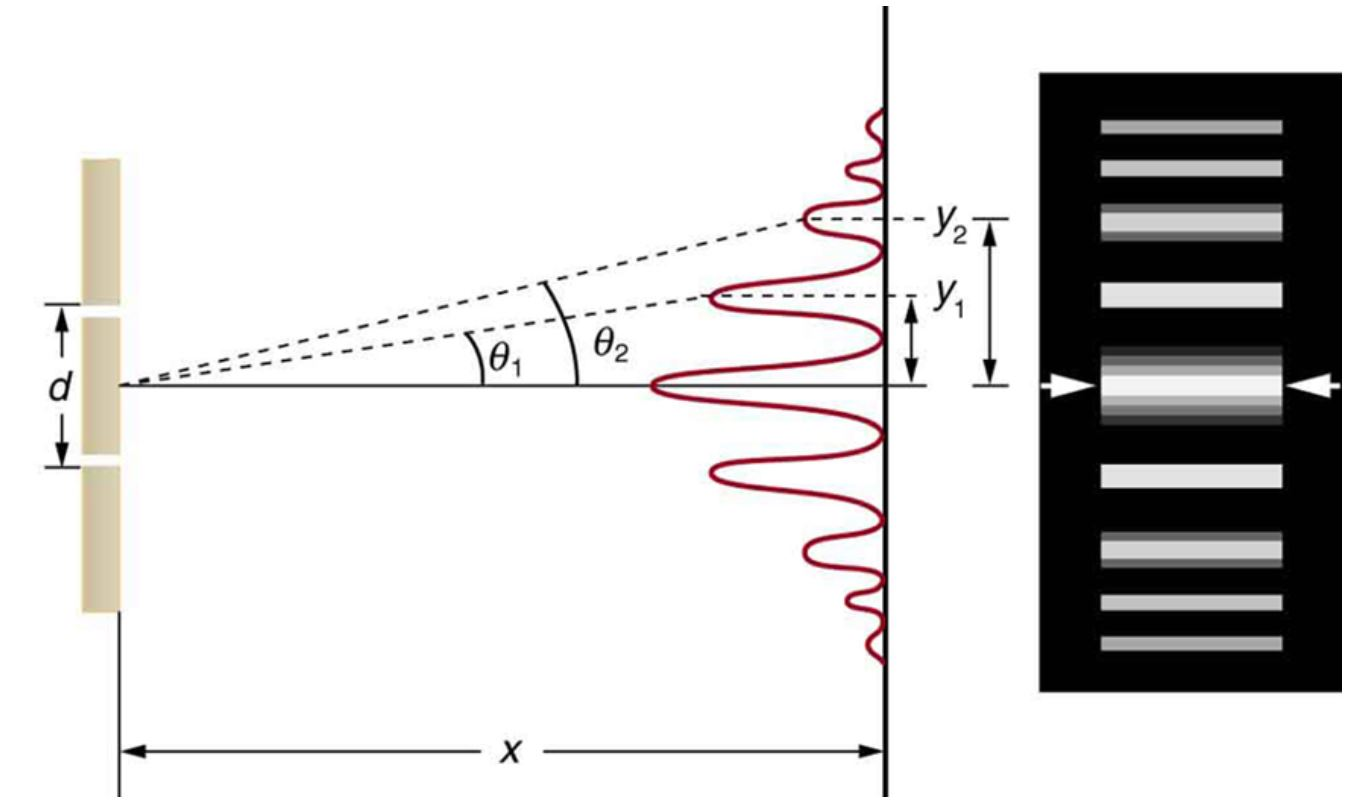
\includegraphics[height=6cm, width=12cm]{1.JPG}

  There is a series of bright and dark bands or fringes. Consider the bright spot in the middle. The light from each split
  has to travel the same distance to reach that point and hence both waves arrive in phase that means crests with crests 
  and troughs with troughs so they add together and create an interference maximum bright spots but if you look slightly 
  to the left there is a dark spot that is because light from one slip has to travel on an angle and it has to travel 
  an extra half a wavelength compared to the light from the other slit which means when one light is arriving as a crest 
  the light from the other slit is arriving as a trough and so they cancel each other out but if you go further left, 
  you see another bright spot because now the like from one of the slits has to travel full extra wavelengths compared to 
  the lights and the other slit and so again they arrive in phase. Crests with crests and troughs with troughs create 
  constructive interference and so we see a bright spot of light and that's how the whole pattern is created.
  
  This experiment gets even more interesting when we decrease the intensity so much that there is not a whole wave of 
  light going through. Like only single photons then how could they interfere with each other because there is only one 
  in the device at any one time. Would we still see an interference pattern? By plotting a graph of the number of photons
  counted as a function of position across the detector, if we have a look at the result over a period of time, we can 
  clearly see that the same interference pattern that we get when we send a ton of photons through but we are getting 
  it out of a single photon. How could this be happening? How could a single photon pass through both slits? Well 
  interpreting these results in terms of the objects we see around ourselves on a daily basis, then the result does not 
  make sense. So we can say that a photon is something different. It is not a wave and it is not a particle, It is a 
  \emph{quantum mechanical object}! Sometimes it seems it has properties of wave and sometimes it seems it has properties
  of a particle. This is one of the reasons photons are counterintuitive. Can we say light is a wave or a particle? 

  \vspace{20px}


  \textbf{III. Theory}

  \vspace{10px}

  % STUFF GOES HERE
  
  \pagebreak


  \textbf{IV. Experimental Procedure}

  \vspace{10px}

  We just followed the given steps in the lab. We learned about the equipment used in the experiment followed
  by the inital steps provided to us. Sadly, the single-photon detector was not working, so 
  we used the given data for this lab report by Dr.Chamberlin. \textcite{Four} 
  
  \begin{figure}[h!]
    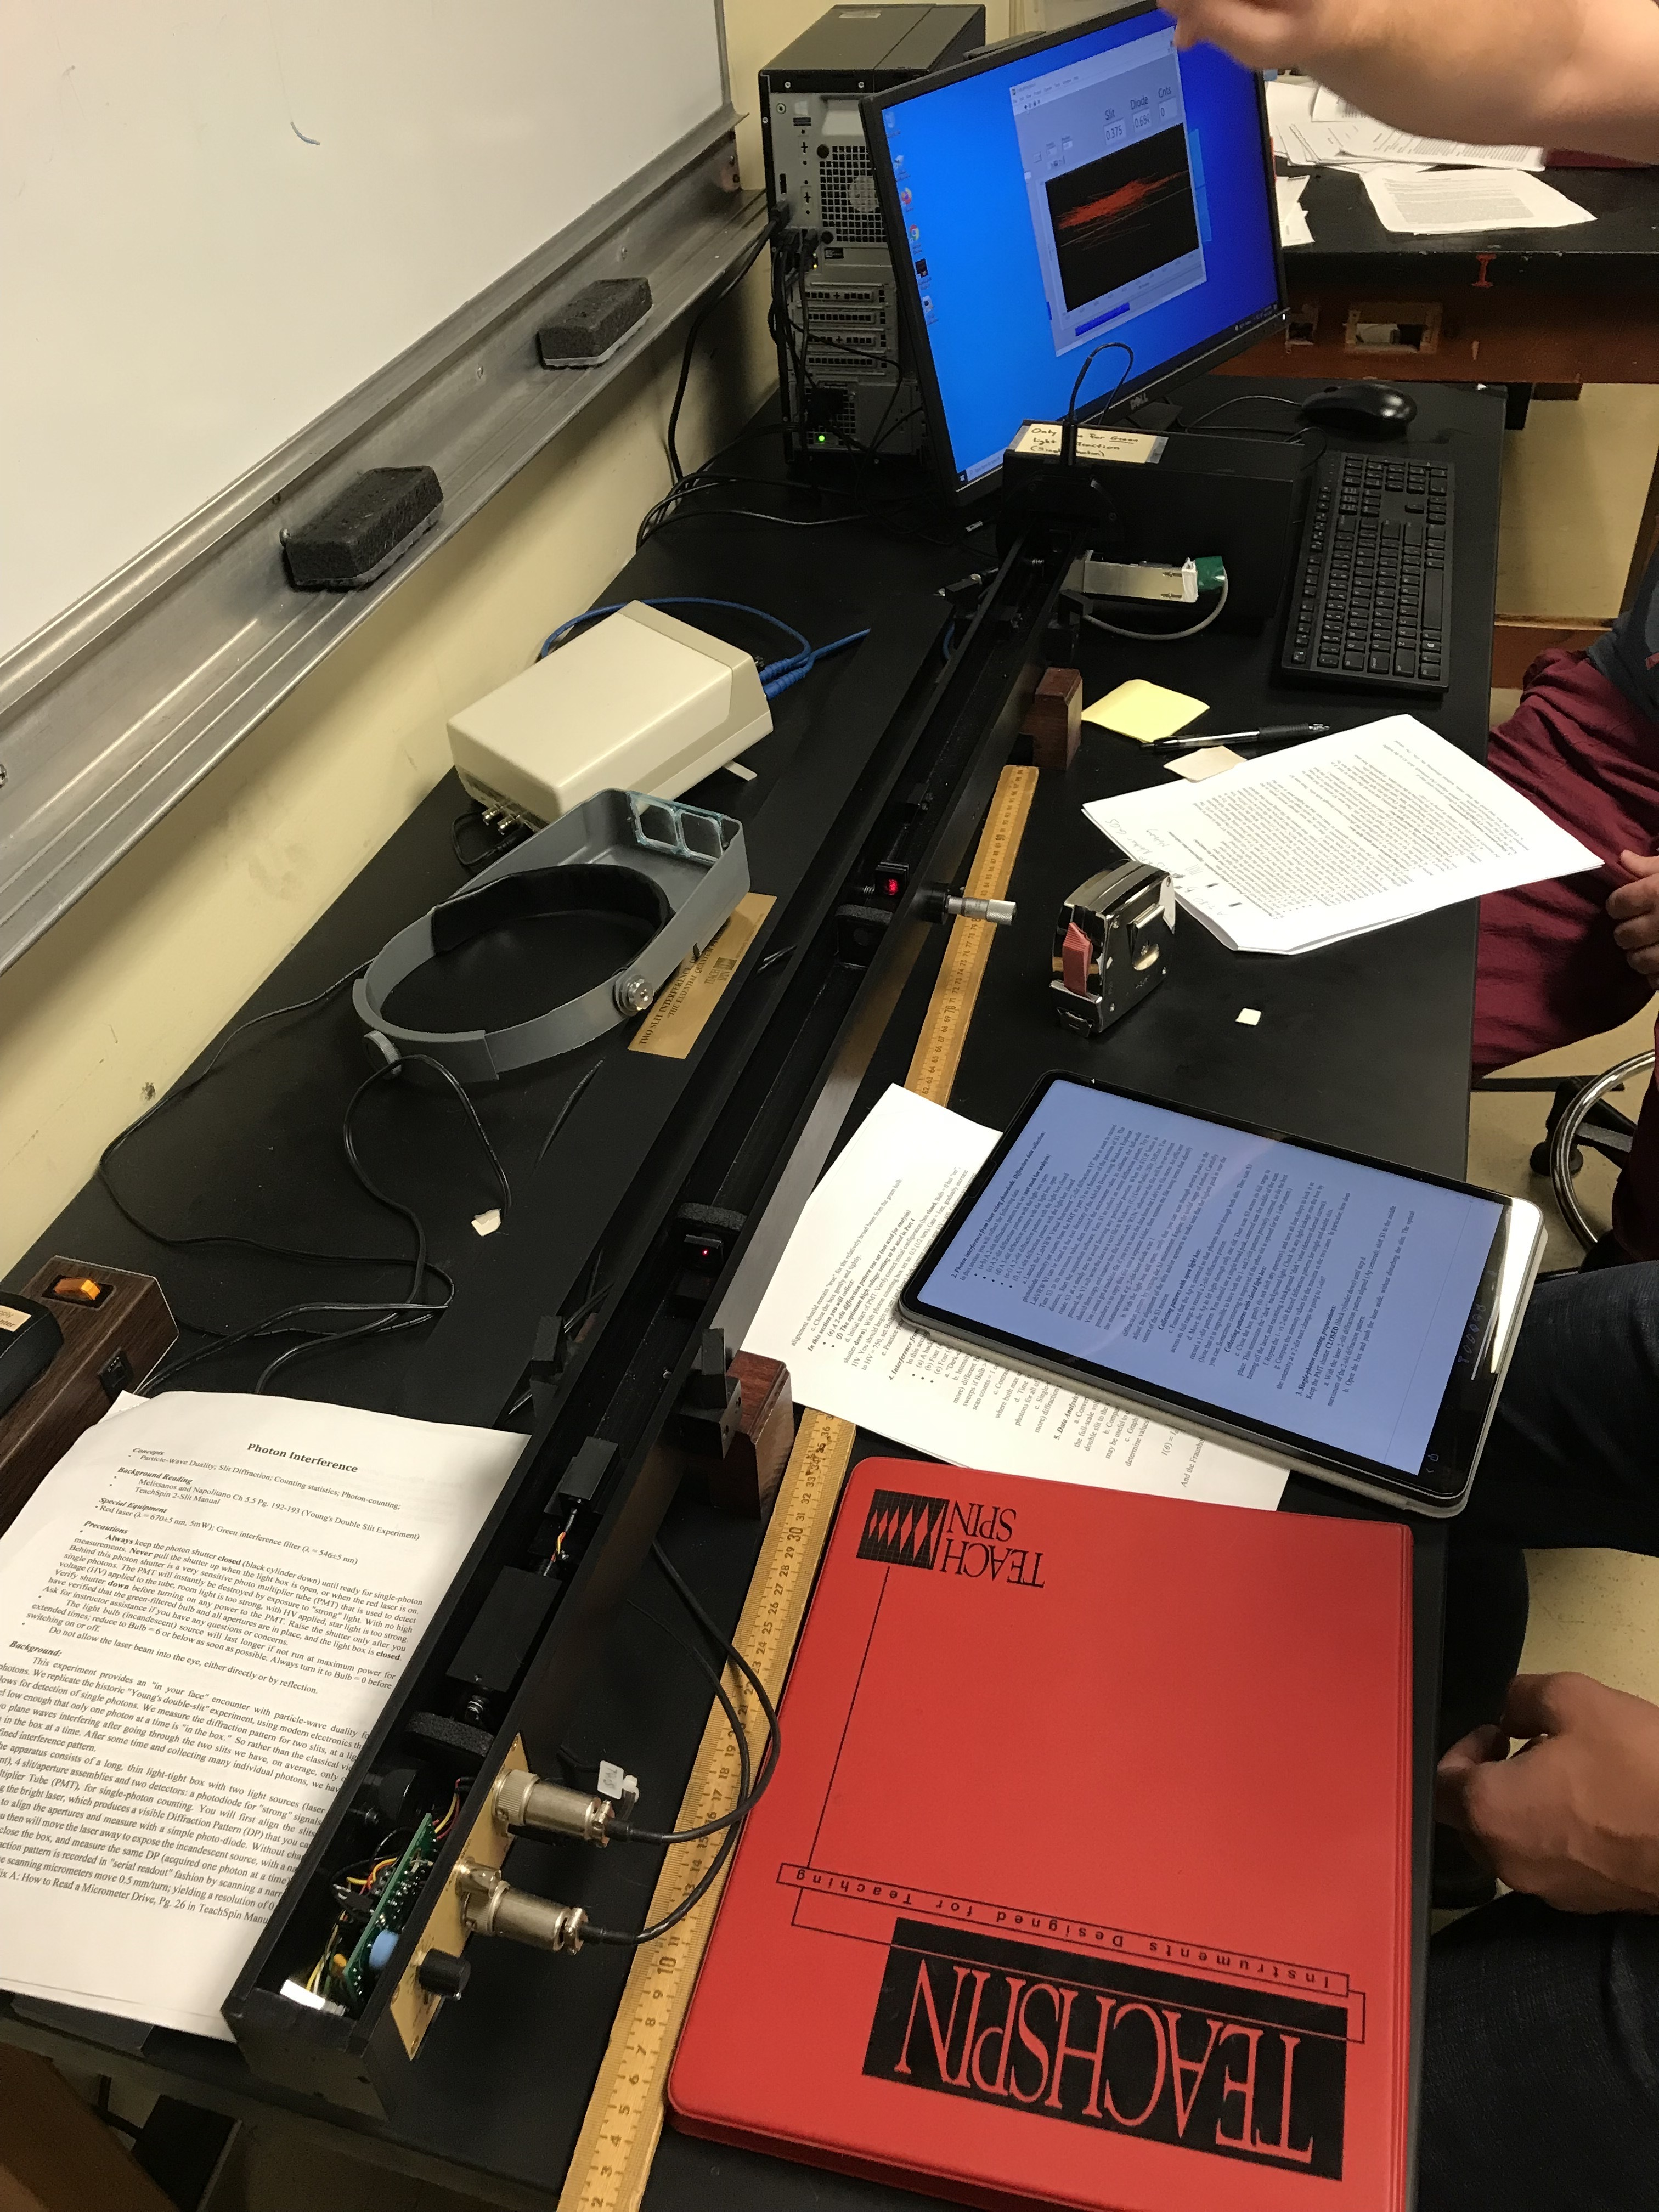
\includegraphics[height=5cm, width=9cm]{2 (1).jpg}
    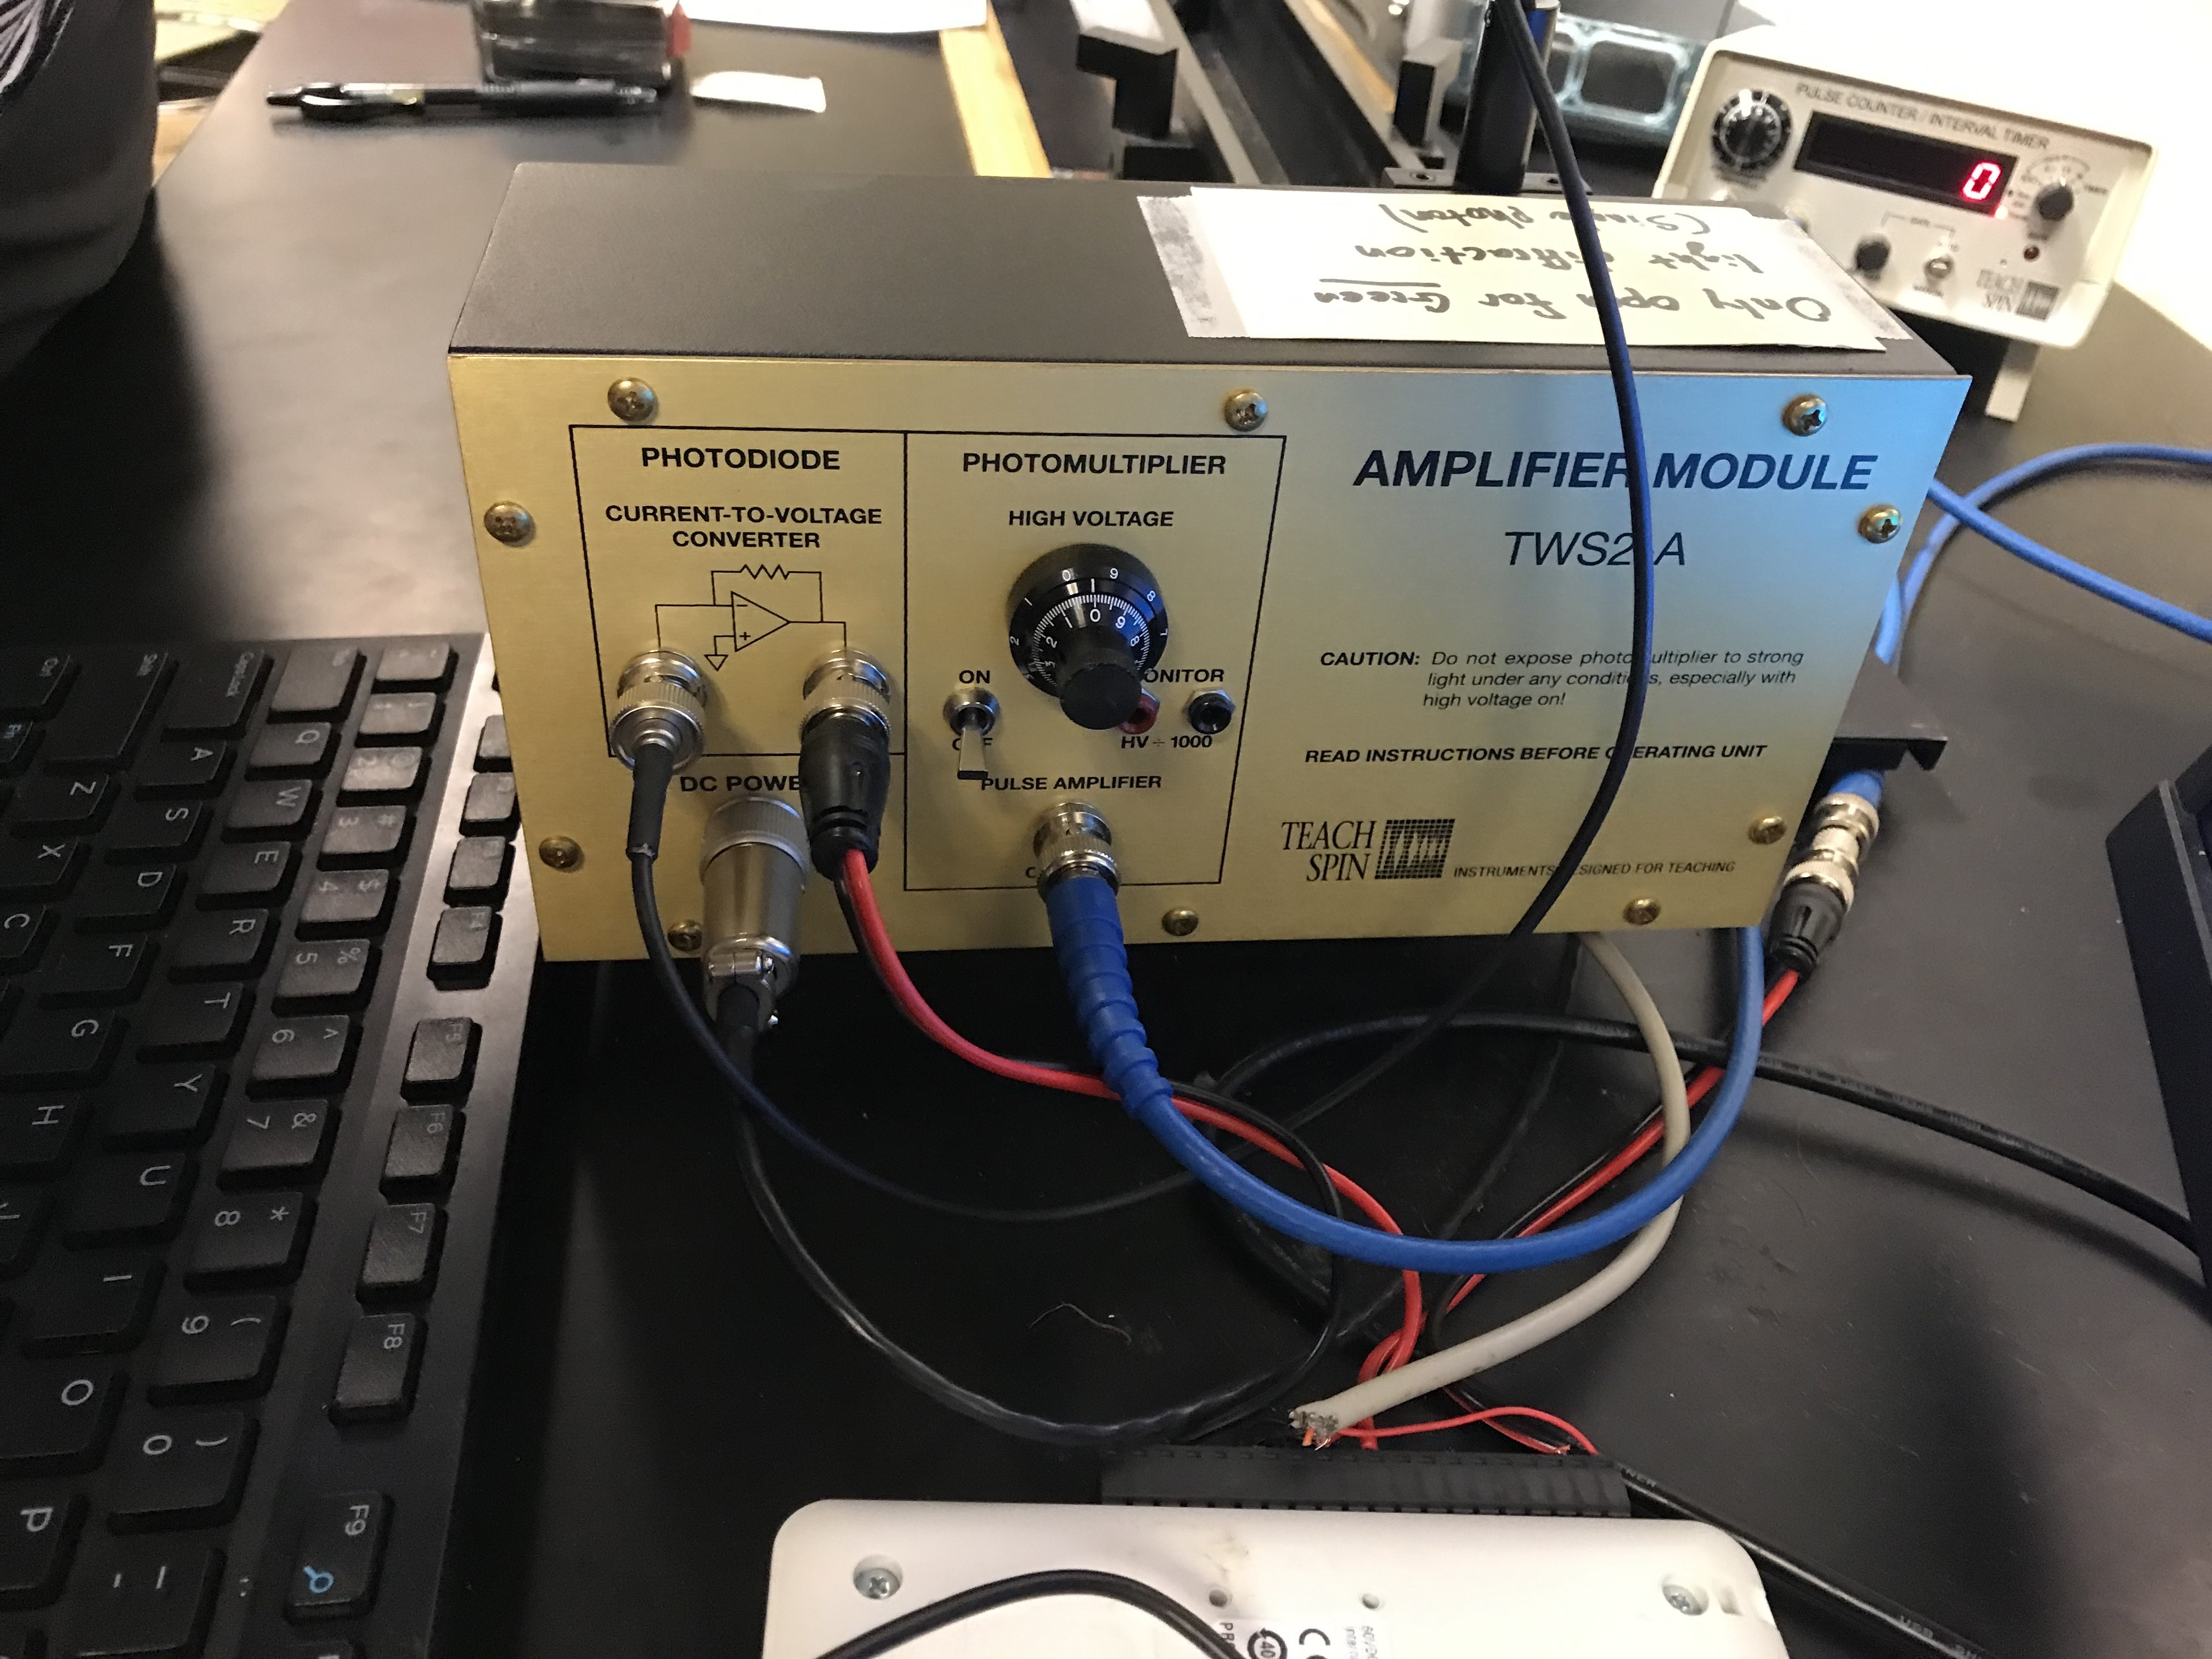
\includegraphics[height=5cm, width=9cm]{2 (2).jpg}
    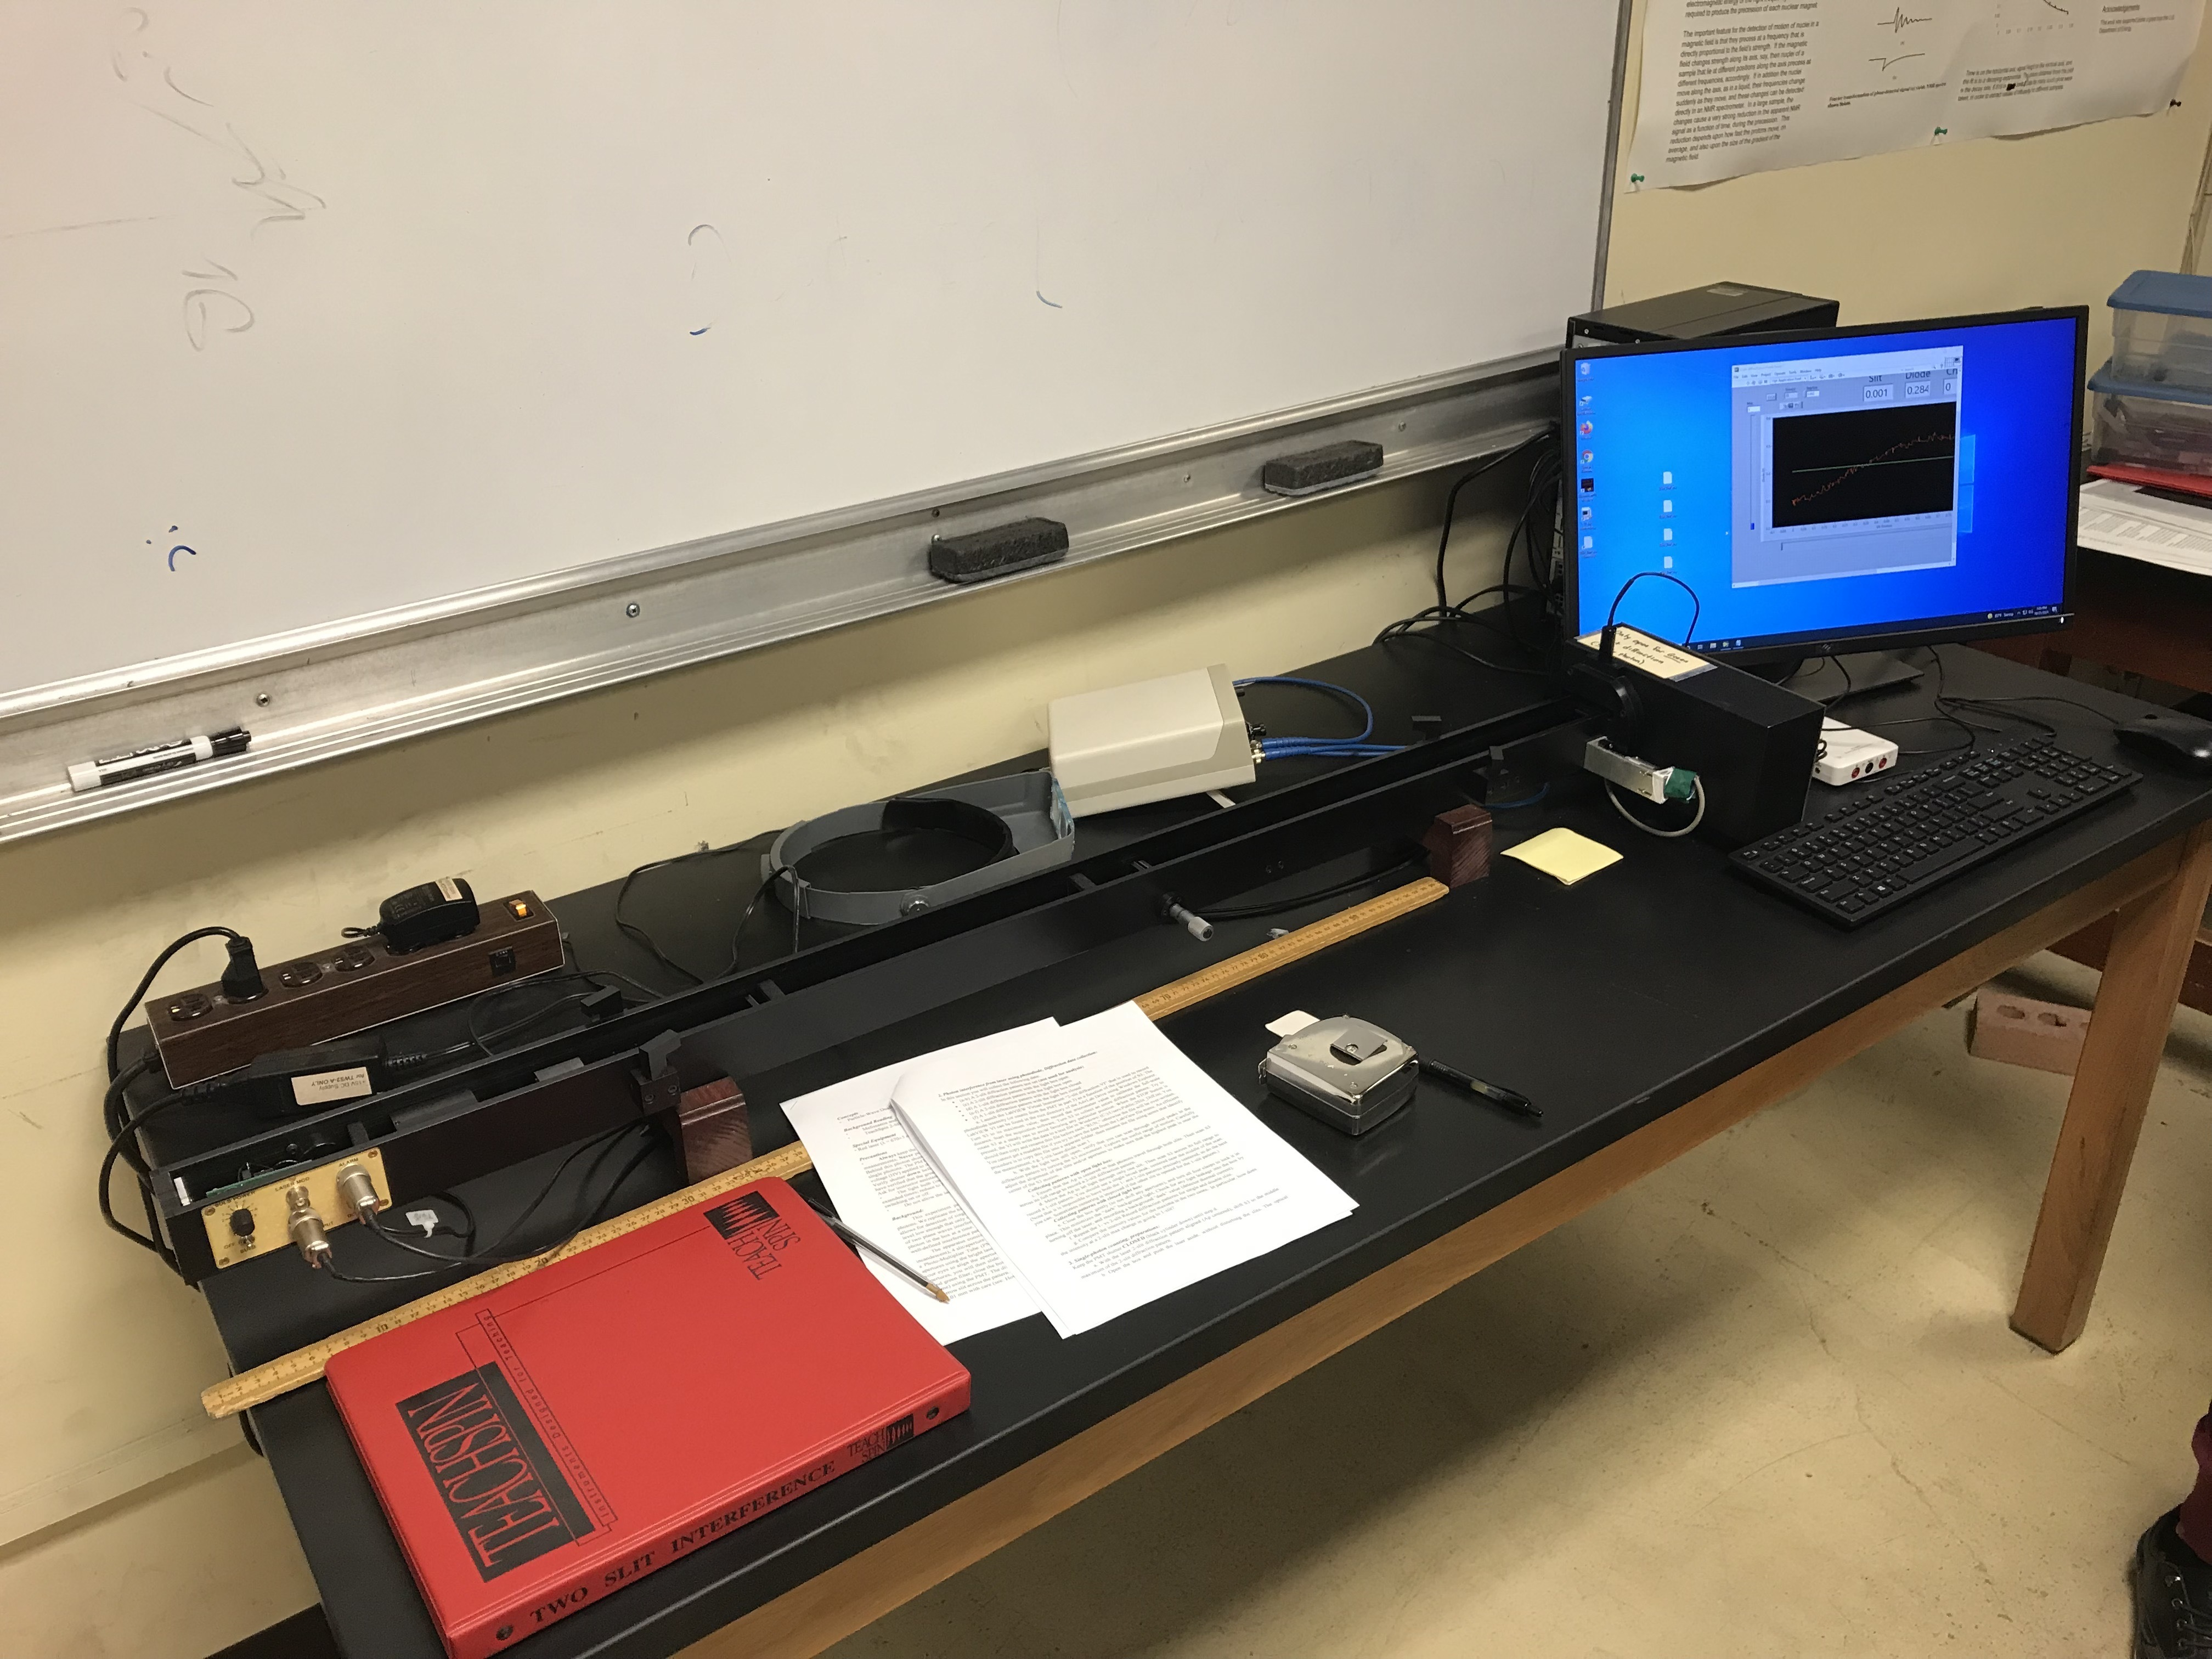
\includegraphics[height=5cm, width=9cm]{2 (3).jpg}
    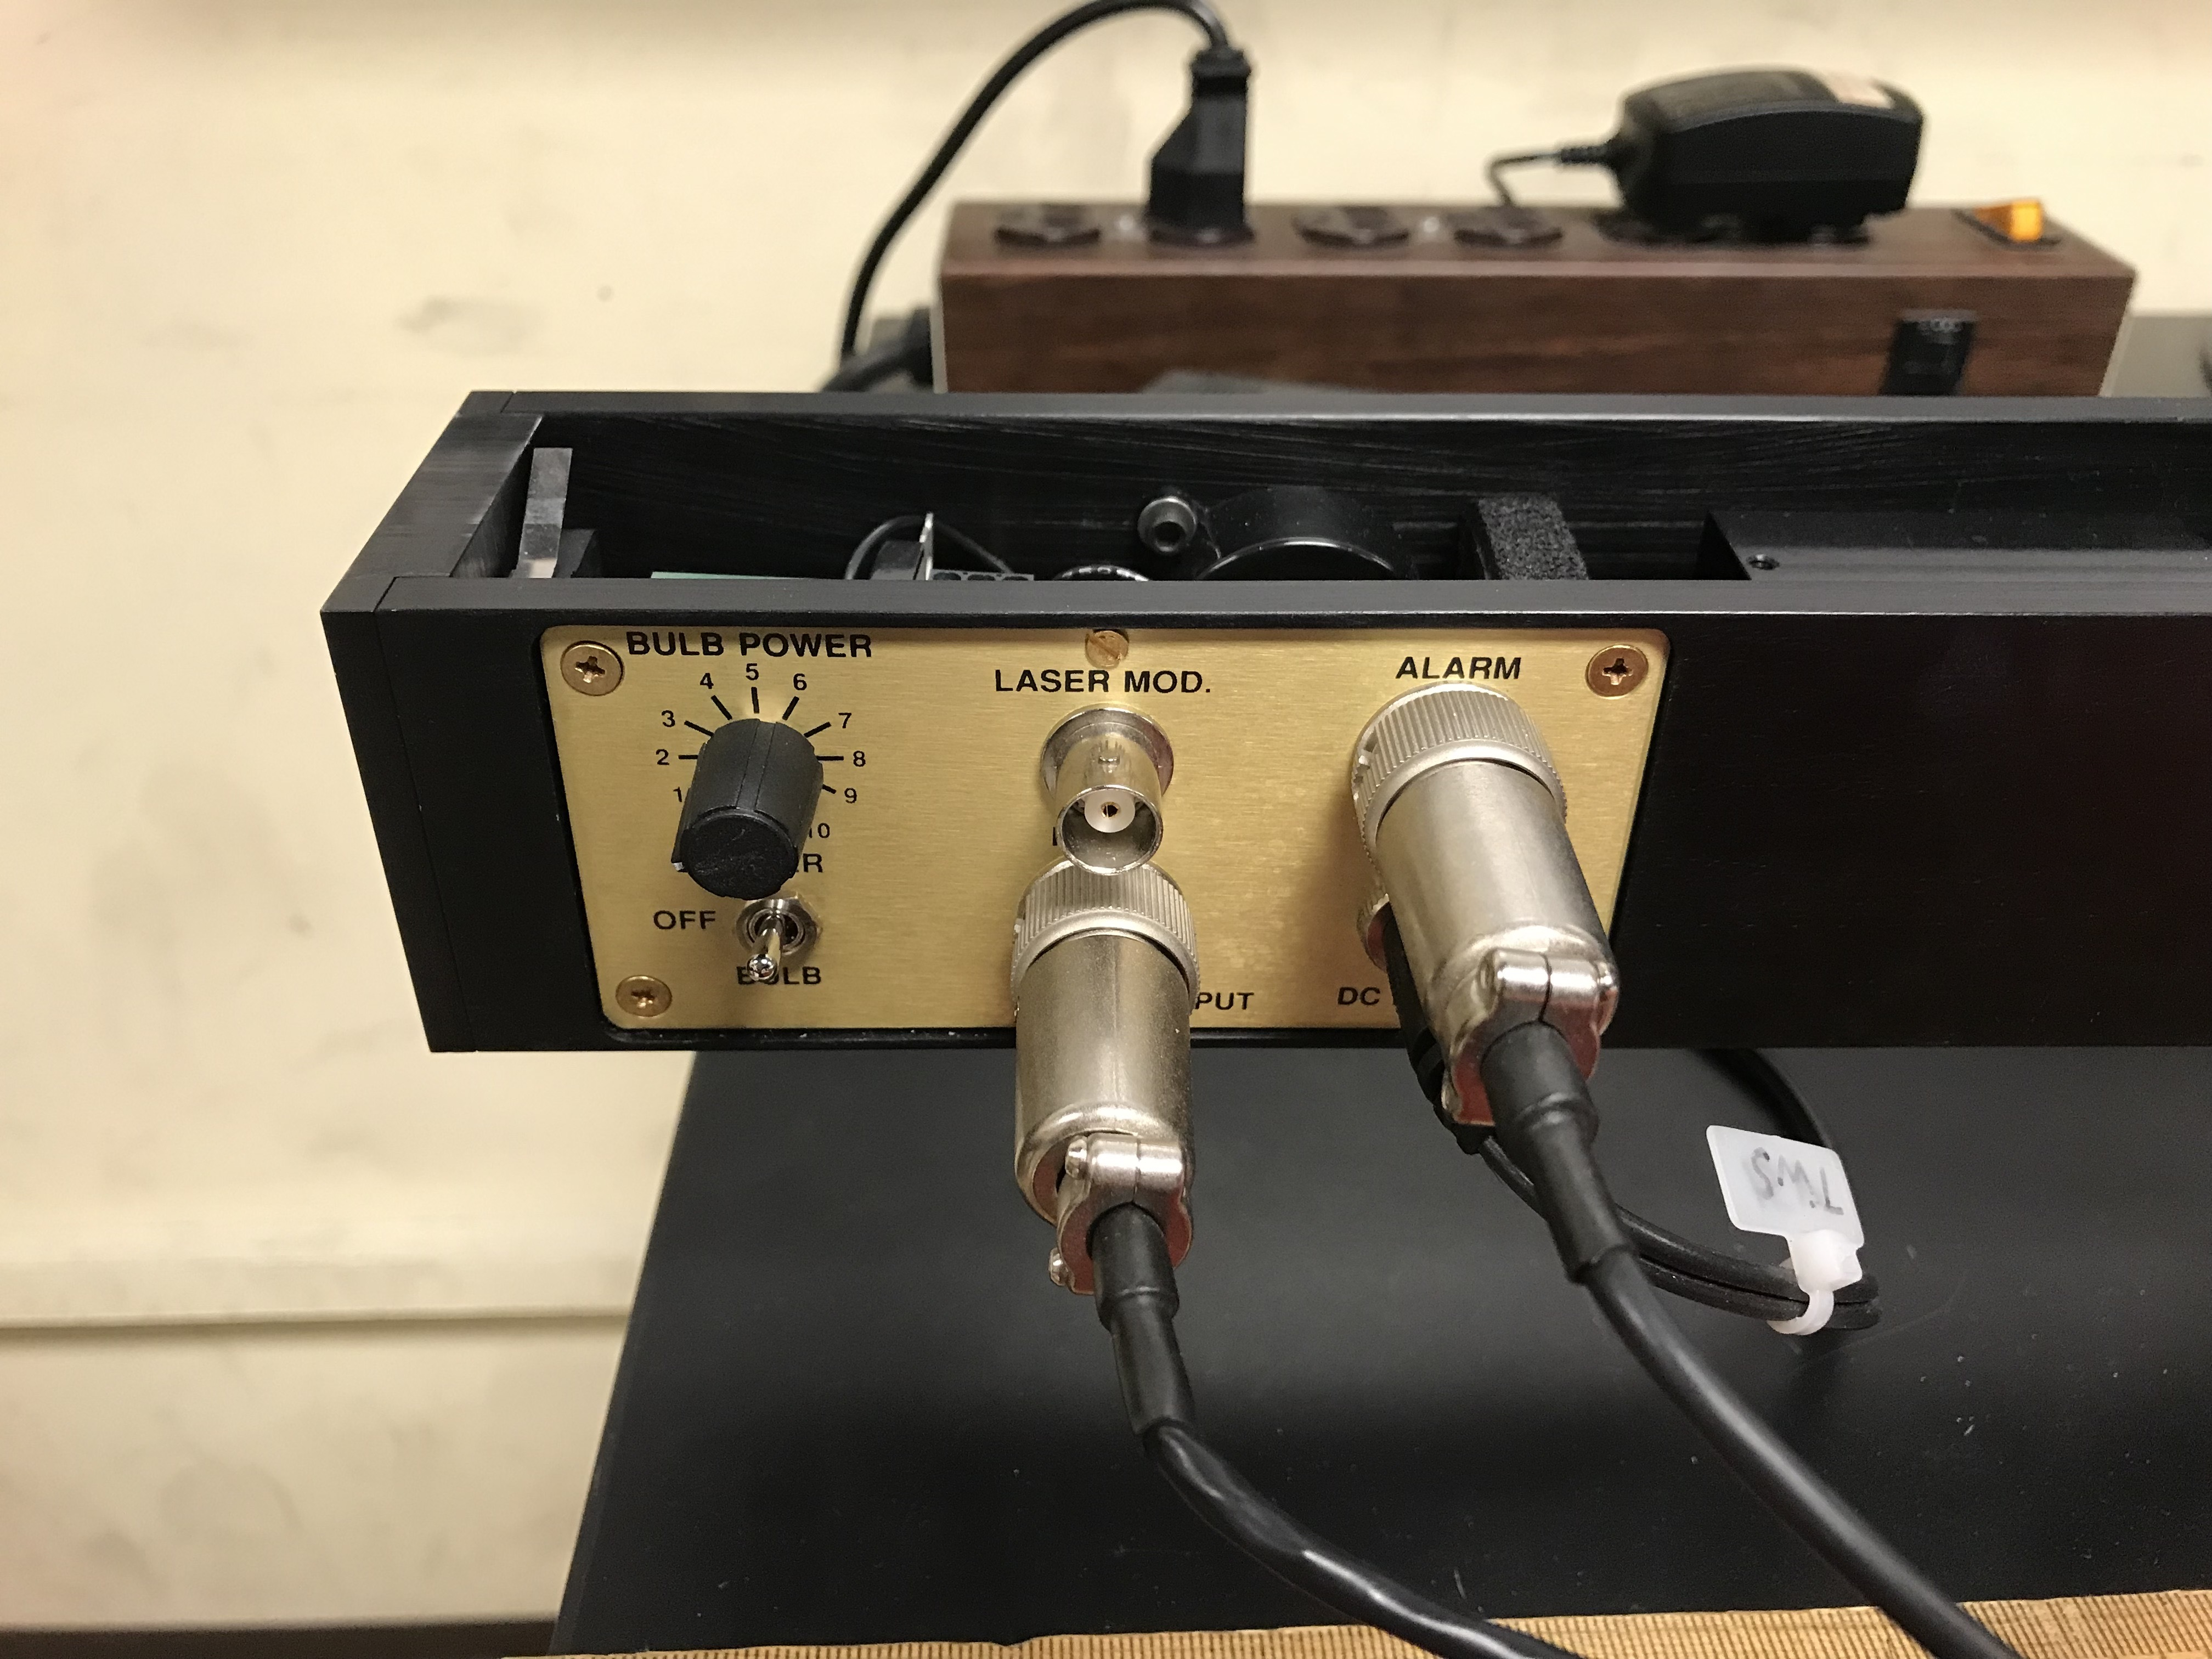
\includegraphics[height=5cm, width=9cm]{2 (4).jpg}
    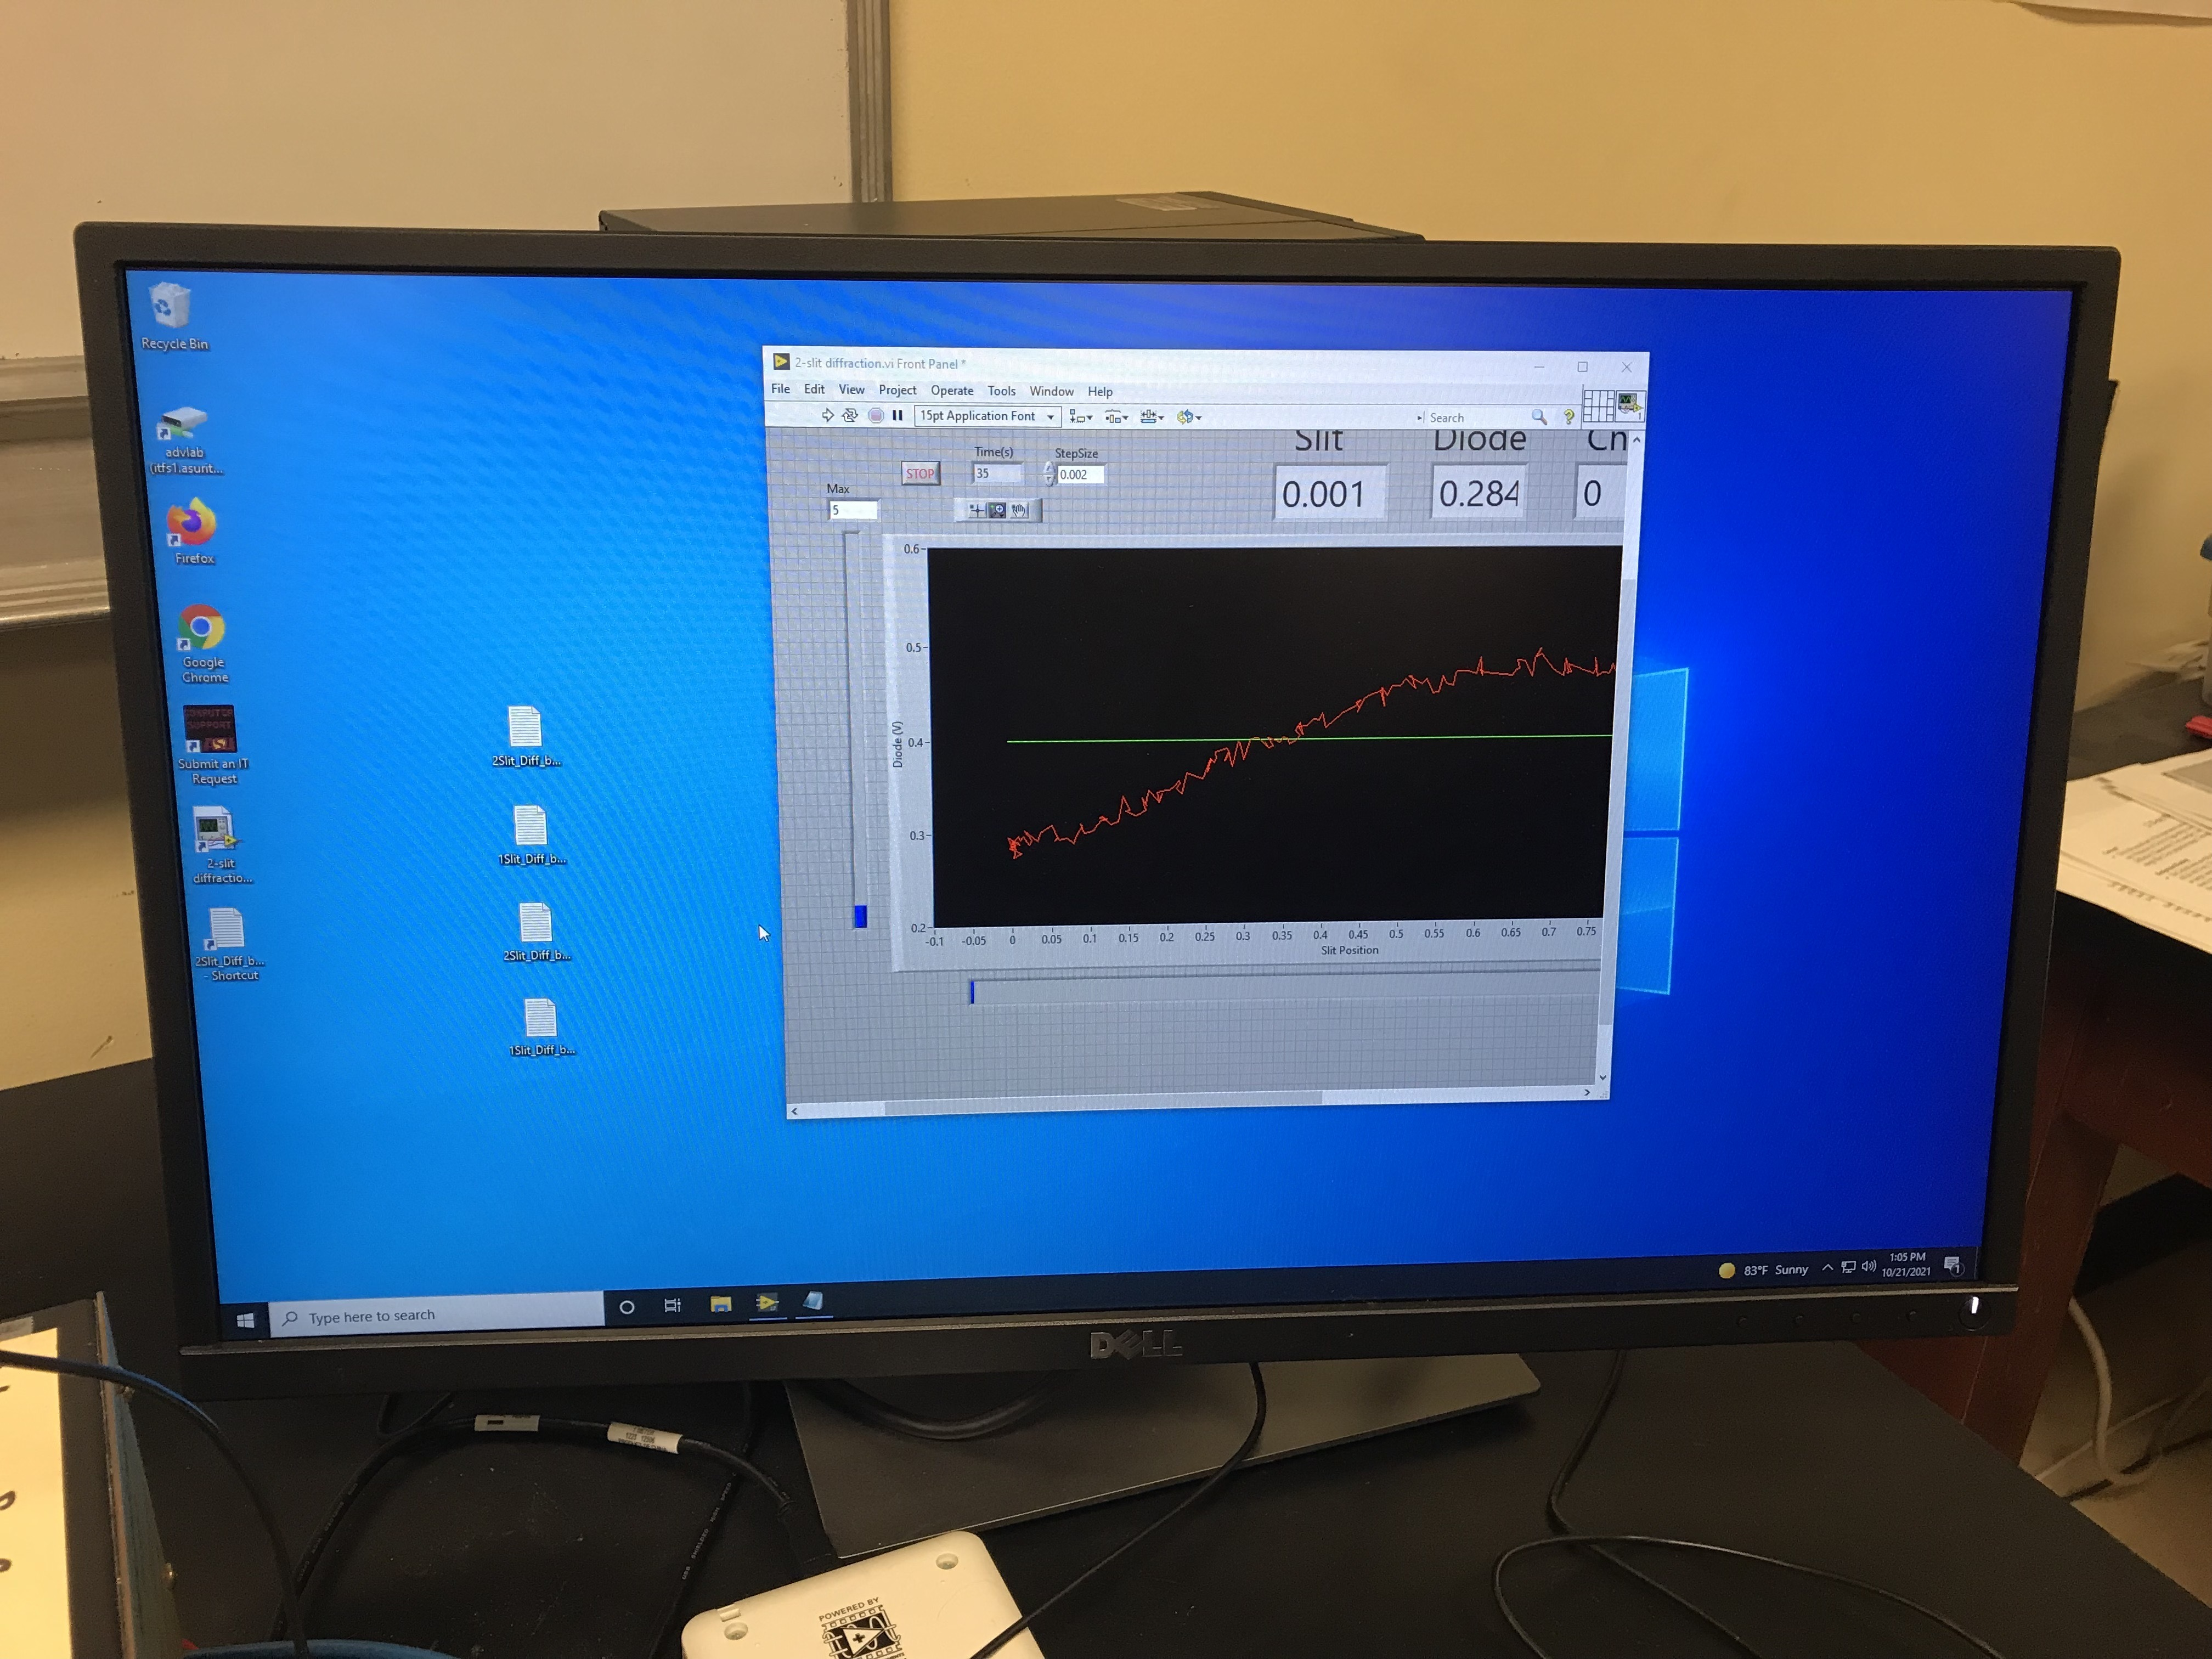
\includegraphics[height=5cm, width=9cm]{2 (5).jpg}
    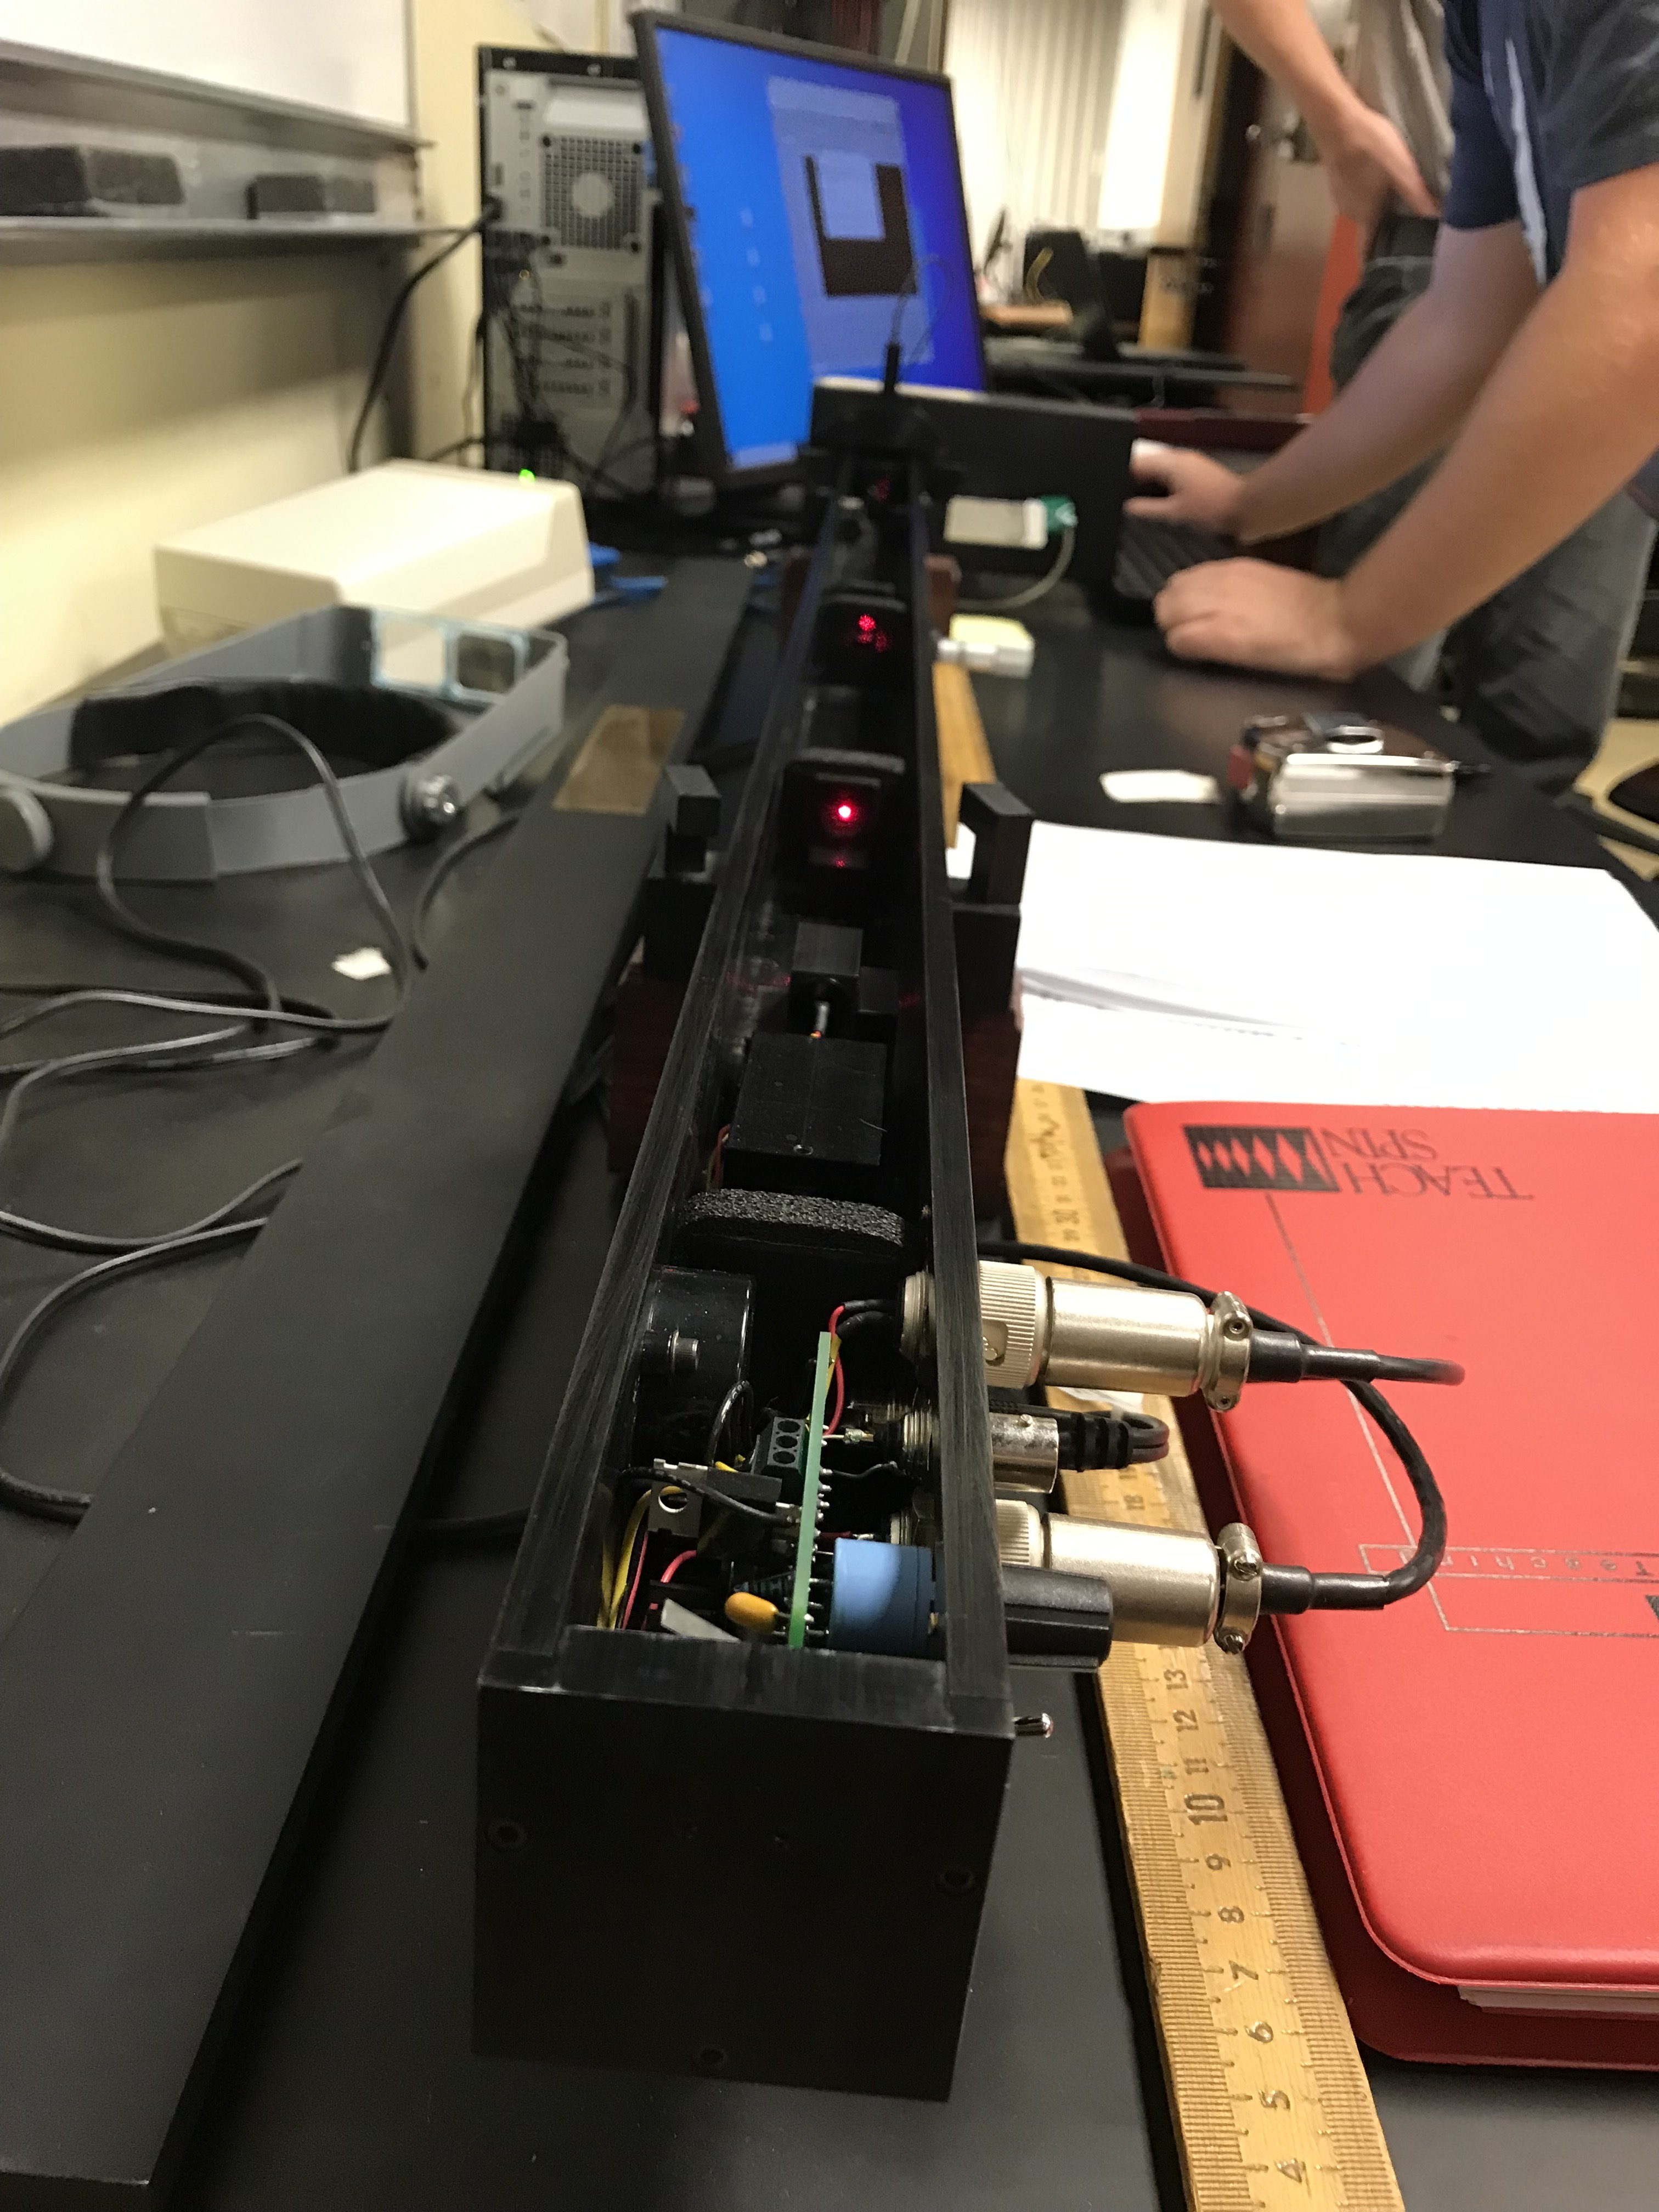
\includegraphics[height=5cm, width=9cm]{2 (6).jpg}
    \caption{
      Some pictures from our experiment.
    }
  \end{figure}

  We have a light source a laser beam. Instead of having two light sources we shine the laser through a
  screen that has two slits which they act like the two sources of waves. From the two slits the light
  shines onto the screen so we are able to see the pattern of constructive and destructive interference 
  of the light waves.
  
  \vspace{20px}


  \textbf{V. Results}

  \vspace{10px}

  Here we go
  
  \vspace{20px}


  \textbf{VI. Discussion}

  \vspace{10px}

  % STUFF GOES HERE
  
  \vspace{20px}


  \textbf{VII. Conclusions}

  \vspace{10px}

  % STUFF GOES HERE
  
  \vspace{20px}


  \printbibliography

\end{document}
